\section{Prácticos realizados}
\subsection{BCD $\rightarrow$ Exceso-3}
\textbf{Consigna:}
Diseñar y armar un conversor de código BCD a XS3 (exceso 3). Realizar: \begin{enumerate} \item Tabla de verdad \item Obtener las funciones lógicas de calidas con circuitos combinacionales. \item Minimizar el circuito y verificar su funcionamiento en el MiniLab. \item Armar el circuito y verificar su funcionamiento en el simular ''falstad.com'' \end{enumerate}

\subsection{Comparador binario}

El siguiente circuito es un comparador binario de dos números $A$ y $B$ de dos bits cada uno. Las salidas ($S0$, $S1$ y $S2$) representan la salida del comparador y cuando $S0 = 1$ cuando $A>B$ y $S2 = 1$ para $A = B$, en caso de no darse la condición, la salida permanece en cero.

\begin{center}
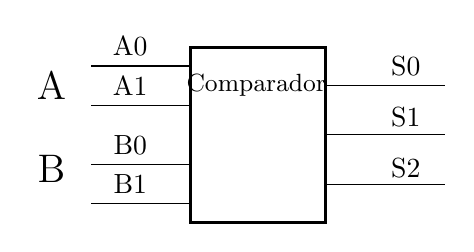
\begin{tikzpicture}
	\node[shape=rectangle, draw, line width=1pt, inner sep=0, minimum width=1.715cm, minimum height=2.215cm] at (5.125, 3.125){};
	\draw (4.25, 4) -- (3, 4);
	\draw (4.25, 3.5) -- (3, 3.5);
	\draw (4.25, 2.25) -- (3, 2.25);
	\draw (4.25, 2.75) -- (3, 2.75);
	\draw (6, 2.5) -- (7.5, 2.5);
	\draw (6, 3.75) -- (7.5, 3.75);
	\draw (6, 3.125) -- (7.5, 3.125);
    \node at (3.5, 4.25) {A0};
    \node at (3.5, 3.75) {A1};
    \node at (3.5, 3) {B0};
    \node at (3.5, 2.5) {B1};
    \node at (7, 4) {S0}; 
    \node at (7, 3.35) {S1};
    \node at (7, 2.7) {S2};
    \node at (5.1 , 3.75) {\small Comparador};
    \node at (2.5, 3.75) {\Large A};
    \node at (2.5, 2.7) {\Large B};
\end{tikzpicture} \end{center}

Se pide:
\begin{enumerate} \item Tabla de verdad. \item Obtener las funciones lógicas de salidas con circuitos combinacionales. \item Circuito mínimo usando mapa de Karnaugh. \item Circuito mínimo usando teoremas y postulados de álgebra de Boole. \item Armado de circuito y verificado en MiniLab. \item Armado de circuito y verificado con simulador ''falstad.com'' \end{enumerate}

\section{Cálculos y respuestas}
\subsection{Exceso 3}
\subsubsection{Tabla de verdad}

\begin{center}
\begin{tabular}{|llll|llll|}
\hline
\rowcolor[HTML]{FFCE93} 
\multicolumn{1}{|c}{\cellcolor[HTML]{FFCE93}\textbf{A}} & \multicolumn{1}{c}{\cellcolor[HTML]{FFCE93}\textbf{B}} & \multicolumn{1}{c}{\cellcolor[HTML]{FFCE93}\textbf{C}} & \multicolumn{1}{c|}{\cellcolor[HTML]{FFCE93}\textbf{D}} & \multicolumn{1}{c}{\cellcolor[HTML]{FFCE93}\textbf{W}} & \multicolumn{1}{c}{\cellcolor[HTML]{FFCE93}\textbf{X}} & \multicolumn{1}{c}{\cellcolor[HTML]{FFCE93}\textbf{Y}} & \multicolumn{1}{c|}{\cellcolor[HTML]{FFCE93}\textbf{Z}} \\ \hline
0                                                       & 0                                                      & 0                                                      & 0                                                       & 0                                                      & 0                                                      & 1                                                      & 1                                                       \\
0                                                       & 0                                                      & 0                                                      & 1                                                       & 0                                                      & 1                                                      & 0                                                      & 0                                                       \\
0                                                       & 0                                                      & 1                                                      & 0                                                       & 0                                                      & 1                                                      & 0                                                      & 1                                                       \\
0                                                       & 0                                                      & 1                                                      & 1                                                       & 0                                                      & 1                                                      & 1                                                      & 0                                                       \\
0                                                       & 1                                                      & 0                                                      & 0                                                       & 0                                                      & 1                                                      & 1                                                      & 1                                                       \\
0                                                       & 1                                                      & 0                                                      & 1                                                       & 1                                                      & 0                                                      & 0                                                      & 0                                                       \\
0                                                       & 1                                                      & 1                                                      & 0                                                       & 1                                                      & 0                                                      & 0                                                      & 1                                                       \\
0                                                       & 1                                                      & 1                                                      & 1                                                       & 1                                                      & 0                                                      & 1                                                      & 0                                                       \\
1                                                       & 0                                                      & 0                                                      & 0                                                       & 1                                                      & 0                                                      & 1                                                      & 1                                                       \\
1                                                       & 0                                                      & 0                                                      & 1                                                       & 1                                                      & 1                                                      & 0                                                      & 0                                                       \\
1                                                       & 0                                                      & 1                                                      & 0                                                       & X                                                      & X                                                      & X                                                      & X                                                       \\
1                                                       & 0                                                      & 1                                                      & 1                                                       & X                                                      & X                                                      & X                                                      & X                                                       \\
1                                                       & 1                                                      & 0                                                      & 0                                                       & X                                                      & X                                                      & X                                                      & X                                                       \\
1                                                       & 1                                                      & 0                                                      & 1                                                       & X                                                      & X                                                      & X                                                      & X                                                       \\
1                                                       & 1                                                      & 1                                                      & 0                                                       & X                                                      & X                                                      & X                                                      & X                                                       \\
1                                                       & 1                                                      & 1                                                      & 1                                                       & X                                                      & X                                                      & X                                                      & X                                                       \\ \hline
\end{tabular}
\end{center}

\subsubsection{Obtención de funciones lógicas por Karnaugh}

\begin{center}
\begin{Karnaugh}
    \contingut{0,1,1,1,1,0,0,0,X,X,X,X,0,1,X,X}
   % \implicant{1}{3}{red}
   % \implicant{2}{3}{green}
   % \implicant{5}{15}{purple}
   \implicantdaltbaix[3pt]{3}{10}{blue}
   \implicantdaltbaix[3pt]{1}{11}{red}
   \implicant{4}{12}{green}
    % \implicantcantons[2pt]{orange}
   % \implicantcostats{4}{14}{green}
\end{Karnaugh} \end{center}

\ecuacion{X = \sum (1; 2; 3; 4; 9)}
\ecuacion{X = D.\overline{B} + C.\overline{B} + \overline{C}.\overline{D}.B}

\begin{center}
\begin{Karnaugh}
    \contingut{1,0,1,1,1,0,1,1,1,0,X,X,X,X,X,X}
   \implicantcostats{0}{10}{green}
   \implicant{3}{11}{red}
\end{Karnaugh} \end{center}
\newpage
\ecuacion{Y = \sum (0; 3; 4; 7; 8)}
\ecuacion{Y = C.D+\overline{C}.\overline{D}}

\begin{center}
\begin{Karnaugh}
    \contingut{0,0,0,0,0,1,1,1,1,1,X,X,X,X,X,X}
    \implicant{12}{10}{red}
    \implicant{5}{15}{blue}
    \implicant{7}{14}{green}
\end{Karnaugh} \end{center}

\ecuacion{W = \sum (5; 6; 7; 8; 9)}
\ecuacion{W = A + B.D + B.C}

\ecuacion{Z = \sum (0; 2; 4; 6; 8)}
\ecuacion{Z = \overline{D}}

\subsubsection{Implementación y simulación}
\imagen[Implementación con MiniLab]{8cm}{./imagenes/exceso3Minilab.jpg}
\imagen[Circuito simulado en Falstab]{8cm}{./imagenes/simulacionExceso3.jpg}
\begin{center}
\begin{figure}[h!]
\centering
\begin{subfigure}[b]{0.45\linewidth}
\includegraphics[width=\linewidth]{./imagenes/cd4069.png}
\caption{Inversor CD4069 x1}
\end{subfigure}
\begin{subfigure}[b]{0.45\linewidth}
\includegraphics[width=\linewidth]{./imagenes/cd4081.png}
\caption{AND dos entradas x2}
\end{subfigure}
\begin{subfigure}[c]{0.45\linewidth}
\includegraphics[width=\linewidth]{./imagenes/cd4075.png}
\caption{OR tres entradas x1}
\end{subfigure}
\begin{subfigure}[d]{0.45\linewidth}
\includegraphics[width=\linewidth]{./imagenes/cd4071.png}
\caption{OR dos entradas x1}
\end{subfigure}
\caption{Integrados usados}
\end{figure}
\end{center}
\thispagestyle{fancy}

\inicioCodigo{}
\subsubsection{Circuito con compuertas lógicas}
\begin{center}
\begin{tikzpicture}
	% Paths, nodes and wires:
	\draw node[ieeestd not port, rotate=-90] at (4.373, 8.5) {};
	\draw node[ieeestd not port, rotate=-90] at (10.25, 8.515) {};
	\draw node[ieeestd not port, rotate=-90] at (8.25, 8.5) {};
	\draw node[ieeestd not port, rotate=-90] at (6.25, 8.5) {};
	\draw (4.373, 9.377) |- (4.25, 10.25) -- (3.25, 10.25) -- (3.25, 7.75);
	\draw (6.25, 9.5) |- (5.25, 10.25) -- (5.25, 7.75);
	\draw (8.25, 9.377) |- (7.25, 10.25) -| (7.25, 7.5);
	\draw (10.25, 9.392) |- (9.25, 10.25) -- (9.25, 7.5);
	\draw (6.25, 9.377) -| (6.25, 9.5);
	\draw (3.25, 10.25) -| (3.25, 11.25);
	\draw (5.25, 10.25) -| (5.25, 11.25);
	\draw (7.25, 10.25) -| (7.25, 11.25);
	\draw (9.25, 10.25) -| (9.25, 11.25);
	\node[shape=rectangle, draw, line width=1pt, inner sep=0, minimum width=0.965cm, minimum height=0.465cm](Rect1) at (3.25, 11.5){} node[anchor=center] at (Rect1.center){$A$};
	\node[shape=rectangle, draw, line width=1pt, inner sep=0, minimum width=0.965cm, minimum height=0.465cm](Rect2) at (5.25, 11.5){} node[anchor=center] at (Rect2.center){$B$};
	\node[shape=rectangle, draw, line width=1pt, inner sep=0, minimum width=0.965cm, minimum height=0.465cm](Rect3) at (7.25, 11.5){} node[anchor=center] at (Rect3.center){$C$};
	\node[shape=rectangle, draw, line width=1pt, inner sep=0, minimum width=0.965cm, minimum height=0.465cm](Rect4) at (9.25, 11.5){} node[anchor=center] at (Rect4.center){$D$};
	\draw node[american and port] (N1) at (12.886, 6.97) {} node[anchor=south] at (N1.north){$B.D$};
	\draw node[american and port] (N2) at (12.886, 5.28) {} node[anchor=south] at (N2.north){$B.C$};
	\draw node[ieeestd or port] at (15.5, 6.28) {};
	\draw node[ieeestd or port] (N3) at (18.169, 4.53) {} node[anchor=west] at (N3.east){$W$};
	\draw (5.25, 7.75) -| (5.25, 7.25) -- (11.5, 7.25);
	\draw (11.5, 6.69) -| (9.25, 6.75) -| (9.25, 7.5);
	\draw (5.25, 5) -| (5.25, 7.25);
	\draw (11.5, 5) |- (5.25, 5);
	\draw (11.5, 5.56) -| (7.25, 7.5);
	\draw (14.419, 6) |- (13.75, 6) |- (13.04, 5.28);
	\draw (14.419, 6.56) -| (13.75, 6.75) |- (13.04, 6.97);
	\draw (3.25, 7.75) |- (17.088, 4.25);
	\draw (17.088, 4.81) -| (16.581, 6.28);
	\draw node[american and port] (N4) at (12.886, 3.22) {} node[anchor=south] at (N4.north){$D.\overline{B}$};
	\draw node[american and port] (N5) at (12.886, 1.47) {} node[anchor=south] at (N5.north){$C.\overline{B}$};
	\draw (11.5, 3.5) |- (9.25, 3.5) -| (9.25, 6.75);
	\draw (11.5, 2.94) -| (6.25, 3);
	\draw (6.25, 3) -- (6.25, 7.623);
	\draw (11.5, 1.75) -| (7.25, 5.56);
	\draw (11.5, 1.19) -| (6.25, 3);
	\draw node[american and port] (N6) at (13, -0.25) {} node[anchor=south] at (N6.north){$\overline{C}.\overline{B}$};
	\draw node[american and port] (N7) at (15.636, -0.97) {} node[anchor=south] at (N7.north){$\overline{C}.\overline{D} .B$};
	\draw (11.614, 0.03) -| (8.25, 7.623);
	\draw (11.614, -0.53) -| (6.25, 1.19);
	\draw (14.25, -0.69) -| (13.5, -0.25) |- (13.154, -0.25);
	\draw (14.25, -1.25) -| (5.25, 5);
	\draw node[ieeestd or port] at (14.723, 2.47) {};
	\draw (13.04, 1.47) -| (13.641, 2.19);
	\draw (13.641, 2.75) |- (13.04, 3.22);
	\draw node[ieeestd or port] (N8) at (18.223, 1.03) {} node[anchor=west] at (N8.east){$X$};
	\draw (17.141, 1.31) -| (15.804, 2.47);
	\draw (15.79, -0.97) -| (17.141, 0.75);
	\draw node[american and port] (N9) at (13.136, -2.78) {} node[anchor=south] at (N9.north){$\overline{C}.\overline{D}$};
	\draw (11.75, -2.5) -| (10.25, 7.75);
	\draw (11.75, -3.06) -| (8.25, 0.03);
	\draw node[american and port] (N10) at (13.136, -4.47) {} node[anchor=south] at (N10.north){$C.D$};
	\draw (11.75, -4.19) -| (7.25, 1.75);
	\draw (11.75, -4.75) -| (9.25, 3.5);
	\draw node[ieeestd or port] (N11) at (15.581, -3.53) {} node[anchor=west] at (N11.east){$Y$};
	\draw (13.29, -2.78) -| (14.5, -3.25);
	\draw (14.5, -3.81) |- (13.29, -4.47);
	\draw node[ieeestd buffer port] (N12) at (15.377, -6.25) {} node[anchor=west] at (N12.east){$Z$};
	\draw (14.5, -6.25) -| (9.25, -4.75);
\end{tikzpicture}
\end{center}
\finalCodigo{}
\thispagestyle{fancy}

\subsection{Comparador binario}
\ecuacion{S_0 = 1 \rightarrow A > B}
\ecuacion{S_1 = 1 \rightarrow A < B}
\ecuacion{S_2 = 1 \rightarrow A = B}

\subsubsection{Tabla de verdad}
\begin{center}
\begin{tabular}{|cccc|ccc|}
\hline
\rowcolor[HTML]{FFCCC9} 
\textbf{$A_1$} & \textbf{$A_0$} & \textbf{$B_1$} & \multicolumn{1}{l|}{\cellcolor[HTML]{FFCCC9}\textbf{$B_0$}} & \textbf{$S_0$} & \textbf{$S_1$} & \textbf{$S_2$} \\ \hline
0              & 0              & 0              & 0                                                           & 0              & 0              & 1              \\
0              & 0              & 0              & 1                                                           & 0              & 1              & 0              \\
0              & 0              & 1              & 0                                                           & 0              & 1              & 0              \\
0              & 0              & 1              & 1                                                           & 0              & 1              & 0              \\
0              & 1              & 0              & 0                                                           & 1              & 0              & 0              \\
0              & 1              & 0              & 1                                                           & 0              & 0              & 1              \\
0              & 1              & 1              & 0                                                           & 0              & 1              & 0              \\
0              & 1              & 1              & 1                                                           & 0              & 1              & 0              \\
1              & 0              & 0              & 0                                                           & 1              & 0              & 0              \\
1              & 0              & 0              & 1                                                           & 1              & 0              & 0              \\
1              & 0              & 1              & 0                                                           & 0              & 0              & 1              \\
1              & 0              & 1              & 1                                                           & 0              & 1              & 0              \\
1              & 1              & 0              & 0                                                           & 1              & 0              & 0              \\
1              & 1              & 0              & 1                                                           & 1              & 0              & 0              \\
1              & 1              & 1              & 0                                                           & 1              & 0              & 0              \\
1              & 1              & 1              & 1                                                           & 0              & 0              & 1              \\ \hline
\end{tabular}
\end{center}
\subsubsection{Obtención de funciones lógicas por Karnaugh}

\begin{center}
\begin{Karnaugh}
    \contingut{0,0,0,0,0,0,0,0,1,1,0,0,1,1,1,0}
    \implicant{12}{9}{red}
    \implicantcostats[3pt]{12}{14}{blue}
\end{Karnaugh} \end{center}

\ecuacion{S_0 = \sum (4;9;15;14;13;12;8)}
\ecuacion{S_0 = (A_0 \cdot \overline{B_1} \cdot \overline{B_0}) + (A_1 \cdot A_0 \cdot \overline{B_0}) +( A_1 \cdot \overline{B_1})}

\begin{center}
\begin{Karnaugh}
    \contingut{0,1,1,1,0,0,1,1,0,0,0,1,0,0,0,0}
    \implicant{1}{3}{red}
    \implicant{1}{6}{green}
    \implicantdaltbaix[3pt]{3}{11}{blue}
\end{Karnaugh} \end{center}

\newpage

\ecuacion{S_1 = \sum (1;2;3;6;7;11)}
\ecuacion{S_1 = (\overline{A_1} \cdot \overline{A_0} \cdot B_0) + (\overline{A_1} \cdot B_1) + (\overline{A_0} \cdot B_1 \cdot B_0)}
\begin{center}
\begin{Karnaugh}
    \contingut{1,0,0,0,0,1,0,0,0,0,1,0,0,0,0,1}
    \implicant{0}{0}{blue}
    \implicant{5}{5}{red}
    \implicant{10}{10}{green}
    \implicant{15}{15}{orange}
\end{Karnaugh} \end{center}

\ecuacion{S_2 = \sum (0;5;10;15)}
\ecuacion{S_2 = (\overline{A_1} \cdot \overline{A_0} \cdot \overline{B_1} \cdot \overline{B_0}) + (\overline{A_1} \cdot A_0 \cdot \overline{B_1} \cdot B_0) + (A_1 \cdot A_0 \cdot B_1 \cdot B_0)}
\ecuacion{+ (A_1 \cdot \overline{A_0} \cdot B_1 \cdot \overline{B_0})}
\ecuacion{XNOR = (\overline{X} \cdot \overline{Y}) + (X \cdot Y)}
\ecuacion{\Rightarrow S_2 = \overline{A_1}\cdot \overline{B_1}(\overline{A_0} \cdot \overline{B_0} + A_0 \cdot B_0) + A_1 \cdot B_1(A_0 \cdot B_0 + \overline{A_0} \cdot \overline{B_0})}
\ecuacion{S_2 = (\overline{A_0} \cdot \overline{B_0} + A_0 \cdot B_0) \cdot (\overline{A_1} \cdot \overline{B_1} + A_1 \cdot B_1)}
\ecuacion{S_2 = \overline{(A_0 \oplus B_0)} \cdot \overline{(A_1 \oplus B_1)}}
\subsubsection{Implementación y simulación}
\imagen[Implementación para el MiniLab]{8cm}{./imagenes/comparadorMinilab.jpg}
\imagen[Circuito para la simulación de Falstab]{8cm}{./imagenes/simulacionComparador.jpg}
\begin{center}
\begin{figure}[h!]
\centering
\begin{subfigure}[b]{0.45\linewidth}
\includegraphics[width=\linewidth]{./imagenes/cd4069.png}
\caption{Inversor CD4069 x1}
\end{subfigure}
\begin{subfigure}[b]{0.45\linewidth}
\includegraphics[width=\linewidth]{./imagenes/cd4081.png}
\caption{AND dos entradas x3}
\end{subfigure}
\begin{subfigure}[c]{0.45\linewidth}
\includegraphics[width=\linewidth]{./imagenes/cd4075.png}
\caption{OR tres entradas x1}
\end{subfigure}
\begin{subfigure}[d]{0.45\linewidth}
\includegraphics[width=\linewidth]{./imagenes/cd4071.png}
\caption{OR dos entradas x1}
\end{subfigure}
\begin{subfigure}[d]{0.45\linewidth}
\includegraphics[width=\linewidth]{./imagenes/cd4077.png}
\caption{XNOR dos entradas x1}
\end{subfigure}

\caption{Integrados usados}
\end{figure}
\end{center}

\thispagestyle{fancy}

\inicioCodigo{}
\subsubsection{Circuito con compuertas lógicas}
\begin{tikzpicture}
	% Paths, nodes and wires:
	\draw node[ieeestd not port, rotate=-90] at (4.373, 8.5) {};
	\draw node[ieeestd not port, rotate=-90] at (10.25, 8.515) {};
	\draw node[ieeestd not port, rotate=-90] at (8.25, 8.5) {};
	\draw node[ieeestd not port, rotate=-90] at (6.25, 8.5) {};
	\draw (4.373, 9.377) |- (4.25, 10.25) -- (3.25, 10.25) -- (3.25, 7.75);
	\draw (6.25, 9.5) |- (5.25, 10.25) -- (5.25, 7.75);
	\draw (8.25, 9.377) |- (7.25, 10.25) -| (7.25, 7.5);
	\draw (10.25, 9.392) |- (9.25, 10.25) -- (9.25, 7.5);
	\draw (6.25, 9.377) -| (6.25, 9.5);
	\draw (3.25, 10.25) -| (3.25, 11.25);
	\draw (5.25, 10.25) -| (5.25, 11.25);
	\draw (7.25, 10.25) -| (7.25, 11.25);
	\draw (9.25, 10.25) -| (9.25, 11.25);
	\node[shape=rectangle, draw, line width=1pt, inner sep=0, minimum width=0.965cm, minimum height=0.465cm](Rect1) at (3.25, 11.5){} node[anchor=center] at (Rect1.center){$A_1$};
	\node[shape=rectangle, draw, line width=1pt, inner sep=0, minimum width=0.965cm, minimum height=0.465cm](Rect2) at (5.25, 11.5){} node[anchor=center] at (Rect2.center){$A_0$};
	\node[shape=rectangle, draw, line width=1pt, inner sep=0, minimum width=0.965cm, minimum height=0.465cm](Rect3) at (7.25, 11.5){} node[anchor=center] at (Rect3.center){$B_1$};
	\node[shape=rectangle, draw, line width=1pt, inner sep=0, minimum width=0.965cm, minimum height=0.465cm](Rect4) at (9.25, 11.5){} node[anchor=center] at (Rect4.center){$B_0$};
	\draw node[american and port] (N1) at (12.75, 7) {} node[anchor=south] at (N1.north){$\overline{B_1}.\overline{B_0}$};
	\draw node[american and port] (N2) at (14.636, 5.78) {} node[anchor=south] at (N2.north){$A_0.\overline{B_1}.\overline{B_0}$};
	\draw (11.364, 7.28) -| (8.25, 7.623);
	\draw (11.364, 6.72) -| (10.25, 7.638);
	\draw (13.25, 6.06) -| (12.904, 7);
	\draw (13.25, 5.5) -| (5.25, 7.75);
	\draw node[american and port] (N3) at (12.846, 4.25) {} node[anchor=south] at (N3.north){$A_0. \overline{B_0}$};
	\draw node[american and port] (N4) at (14.886, 3.03) {} node[anchor=south] at (N4.north){$A_1.A_0. \overline{B_0}$};
	\draw (11.46, 4.53) -| (5.25, 5.5);
	\draw (11.46, 3.97) -| (10.25, 6.75);
	\draw (13, 4.25) -| (13.25, 3.31);
	\draw (13.25, 2.75) -| (3.25, 7.75);
	\draw (13.25, 3.31) -- (13.5, 3.31);
	\draw (13.5, 2.75) |- (13.25, 2.75);
	\draw node[american and port] (N5) at (12.886, 1.22) {} node[anchor=south] at (N5.north){$A_1. \overline{B_1}$};
	\draw (11.5, 1.5) -| (3.25, 2.75);
	\draw (11.5, 0.94) -| (7.25, 7.5);
	\draw node[ieeestd or port] at (16.473, 4.78) {};
	\draw (15.391, 5.06) |- (14.79, 5.78);
	\draw (15.04, 3.03) -| (15.391, 4.5);
	\draw node[ieeestd or port] (N6) at (18.723, 2.47) {} node[anchor=west] at (N6.east){$S_0$};
	\draw (17.641, 2.75) |- (17.554, 4.78);
	\draw (13.04, 1.22) -| (17.641, 2.19);
	\draw node[american and port] (N7) at (12.886, -0.47) {} node[anchor=south] at (N7.north){$B_0.\overline{A_0}$};
	\draw (11.5, -0.19) -| (9.25, 7.5);
	\draw (11.5, -0.75) -| (6.25, 7.623);
	\draw node[american and port] (N8) at (14.886, -1.28) {} node[anchor=south] at (N8.north){$A_1.B_0.\overline{A_0}$};
	\draw node[american and port] (N9) at (13, -2.75) {} node[anchor=south] at (N9.north){$B_0.B_1$};
	\draw (13.5, -1) -- (13.25, -1) |- (13.04, -0.47);
	\draw (13.5, -1.56) -| (3.25, 1.5);
	\draw node[american and port] (N10) at (14.75, -3.5) {} node[anchor=south] at (N10.north){$\overline{A_0}.B_0.B_1$};
	\draw (13.364, -3.22) -| (13.154, -2.75);
	\draw (11.614, -2.47) -| (9.25, -0.19);
	\draw (11.614, -3.03) -| (7.25, 1);
	\draw (13.364, -3.78) -| (6.25, -0.75);
	\draw node[american and port] (N11) at (13, -5) {} node[anchor=south] at (N11.north){$B_1.\overline{A_1}$};
	\draw (11.614, -4.72) -| (7.25, -3.03);
	\draw (11.614, -5.28) -| (4.373, 7.623);
	\draw node[ieeestd or port] at (16.473, -2.28) {};
	\draw (14.904, -3.5) -| (15.391, -2.56);
	\draw (15.391, -2) |- (15.04, -1.28);
	\draw node[ieeestd or port] (N12) at (18.831, -4.03) {} node[anchor=west] at (N12.east){$S_1$};
	\draw (13.154, -5) -| (17.75, -4.31);
	\draw (17.554, -2.28) |- (17.75, -3.75);
	\draw node[american xnor port] (N13) at (13, -6.75) {} node[anchor=south] at (N13.north){$\overline{A_0 \oplus B_0}$};
	\draw node[american xnor port] (N14) at (13, -8.75) {} node[anchor=south] at (N14.north){$\overline{A_1 \oplus B_1}$};
	\draw (11.614, -6.47) -| (5.25, 4.53);
	\draw (11.614, -7.03) -| (9.25, -2.5);
	\draw (11.614, -8.47) -| (3.25, -1.56);
	\draw (11.614, -9.03) -| (7.25, -4.72);
	\draw node[american and port] (N15) at (15, -7.75) {} node[anchor=west] at (N15.east){$S_2$};
	\draw (13.154, -8.75) -| (13.614, -8.03);
	\draw (13.154, -6.75) -| (13.614, -7.47);
\end{tikzpicture}
\finalCodigo{}
\section{Conclusiones}
\subsection{Dificultades enfrentadas}

''La principal dificultad que hemos tenido fue en el desarrollo del mini-laboratorio, ya que quisimos experimentar con el diseño de placas por KiCad y el método casero para hacer placas de circuitos. En cierto punto decidimos frenar y pasar a hacer el mini-laboratorio con protoboards.'' \\
\sangria{}''En cuanto al desarrollo del trabajo práctico, la otra dificultad enfrentada fue la selección de los integrados a usar y la forma de la que íbamos a conectarlos, porque también quisimos experimentar con el uso de placas hechas en casa. Decidimos abandonar brevemente la idea para hacer las conexiones por protoboard, que resultó difícil por sus conecxiones.''

\subsection{Objetivos alcanzados}

''Se logró aplicar lo aprendido sobre mapas de Karnaugh, simplificaciones y circuitos combinacionales para diseñar el BCD-Exceso 3 y el comparador binario, una forma más real de ver las salidas de un sistema.''


